\documentclass[a4paper]{scrreprt}
\usepackage[backend=bibtex,style=numeric]{biblatex}
\usepackage{ngerman}
\usepackage[T1]{fontenc}
\usepackage[utf8]{inputenc}
\usepackage[style=numeric]{biblatex}
\bibliography{../PaperBib}
\usepackage{amsmath}
\usepackage{graphicx}
\usepackage[outdir=../Graphen/]{epstopdf}
\usepackage{textcomp}
\usepackage{floatrow}
\renewcommand{\figurename}{Fig.}
\usepackage{caption}
\setcapindent{0pt}
\usepackage{subcaption}
\usepackage{scrhack}
\usepackage{tabularx}

\newcolumntype{L}[1]{>{\raggedright\arraybackslash}m{#1}}
\newcolumntype{C}[1]{>{\centering\arraybackslash}m{#1}}
\newcolumntype{R}[1]{>{\raggedleft\arraybackslash}m{#1}}


\begin{document}

\title{Improving the modelling of tempo and phoneme duration}
\author{Alexandra Krah}
\date{06. April ~2017}
\maketitle
\chapter*{}
\tableofcontents
\listoffigures

\chapter{Introduction}
Some people speak faster, others speak slower, and all people speak sometimes faster or slower as they usually do. This ``speed`` at which one speaks is what we call ``speech rate``. The fact that we understand people at all natural speech rates is certainly largely due to the quality features of sounds (phonemes) in the given language. However, if we have a perfect audio recording of speech, and play it faster or slower, we immediatly notice how naturalness deteriorates. Synthetic speech shows a similar behaviour when changing the speaking rate. In both cases phoneme quality doesn't need to change. It is its duration that changes, along with some other suprasegmental features like pitch, phrasal accents, etc., and that do the trick. 

The attempts to improve the quality of speech synthesis when tempo changes include linguistic processing, and phoneme length manipulation before the actual synthesis takes place. As mentioned in a patent documentation of Fujitsu Limited, phoneme length manipulation plays an important role in this context and one cannot rely on a linear adjustment function \cite{nishiike2008}. 

\subsection*{Scope}
Phoneme length adjustment is the aspect we wish to adress in this work. In particular, we want to find an algorithm to adjust the phoneme duration according to the speech rate. The resulting phoneme duration should be close to the actual duration that occurs when the speaking rate alters. This would be the same as playing an audio file faster or slower. 

There are several models for phoneme duration approximation, that work pretty well for some languages, German inclusive. However, they consistently don't take the speech rate into consideration, their performance level being acquired within a specific speech rate. When this varies, model performance deteriorates, like van Santen states for his model \cite{Santen1994}. Moreover, all these models have an upper asymptote for their accuracy situated at less than 100\%. It has been suggested, that the influence of so-called ``macroscopic`` \cite{Cummins1999} or para-linguistic \cite{Santen1994} factors should be examined in order to move this asymptote further up. So we focused on speech rate. 

The purpose is therefore not to find another duration approximation model for TTS-systems, but to improve the algorithm of phoneme duration adjustment, given known reference phoneme and word durations, and a target word duration, as presented in Table \ref{tab:Question}. Consequently, the modified speech unit would sound more natural at a faster or a slower speech rate than being modified with a linear function. 

\begin{table}[htbp]
\caption {The challenge} 
\centering
\begin{tabular}{|L{2.5cm}||*{4}{C{.8cm}|}|*{4}{C{.8cm}|}}
	\hline
			& \multicolumn{4}{c||}{ \textit{genau}} & \multicolumn{4}{c|}{ \textit{genau}} \\
	\hline
Phonemes		& g & @ & n & aU & g & @ & n & aU \\
	\hline
Durations (sec) & 0.05 & 0.07 & 0.05 & 0.11 & ?  & ?  & ?  & ? \\
	\hline
Speech rate $dur/\#phon$ & \multicolumn{4}{c||}{0.07} & \multicolumn{4}{c|}{0.11} \\
	\hline
\end{tabular}
\caption*{The first column shows our inputs: duration of each phoneme in German word ``genau``, given a speech rate of 0.07 sec, or a word duration of 0.28 sec. The second column presents our challenge: how long is the duration of each phoneme of the given word, when it is spoken slower, taking e.g. 0.42 sec, speech rate of approx. 0.11 sec?}
\label{tab:Question} 
\end{table}

Hoequist and Kohler observed already back in 1986 that the change in speaking tempo does not produce a linear change of the acoustic segments of an utterance (i. e. phonemes) \cite{Hoequist1986}. Indeed, if one simply ``stretches`` all phonemes in the same manner to accomodate a new speech rate, the result is rather dissapointing, as one can see in Fig. \ref{fig:linear_approx}.

\begin{figure}[htbp]
	\centering
	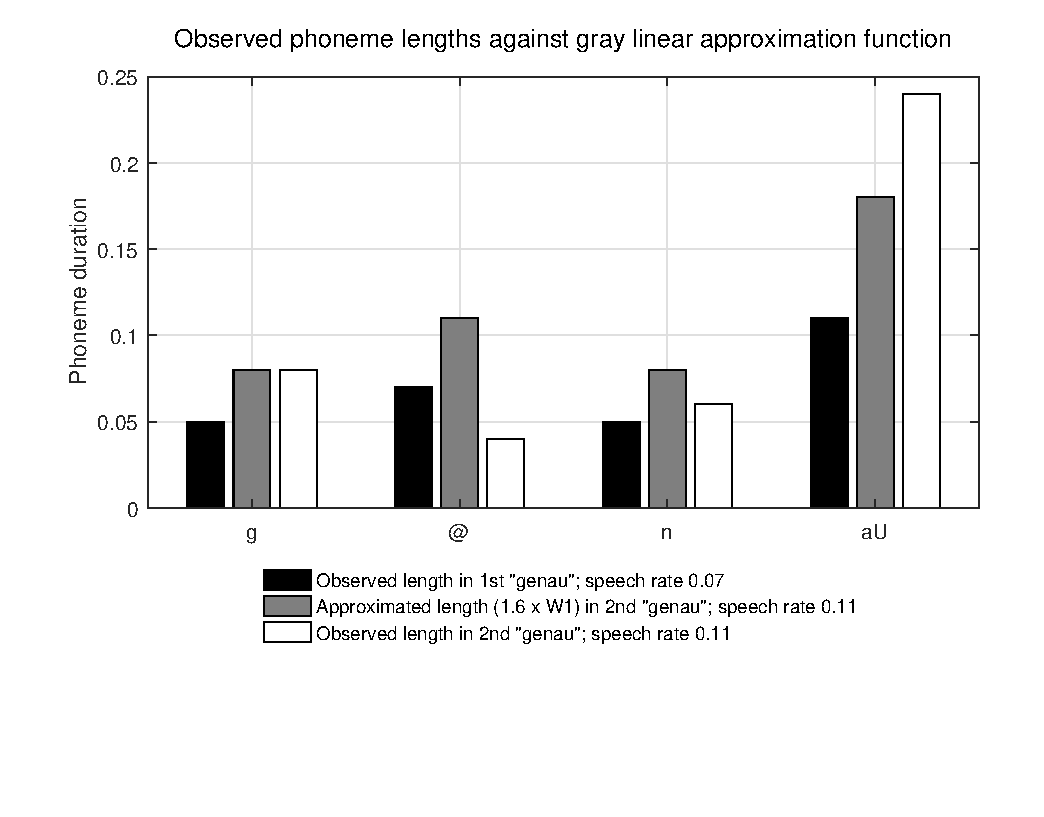
\includegraphics[scale=0.7]{../Graphen/Linear_approx.eps}
	\caption[Linear phoneme duration approximation]{This is a linear solution to the issue presented in table \ref{tab:Question} for the German word ``genau``}
	\label{fig:linear_approx}
\end{figure}

\subsubsection*{Notizen}
Syllable and foot structure of the utternace belong to the important factors influencing the segment length modification  \cite{Hoequist1986}.

More important as the segmentation of the utterance in words is its segmentation in prosodical segments, so-called feet. In spontaneous speech, some word parts may fall, others may be uttered together with other words so that the resulting phoneme duration tends to relate more to the structure of the resulting prosodic segment as to the original word \cite{Kohler1986}. 

Accross the paper we will use the German SAMPA notations when referring to phonemes.

\subsection*{Outline}
We start our approach by defining our methods in chapter 2. In the following chapter we examine our database so that we can proceed with the actual task in chapter 4, where we analyze the German phonemes. We dedicate chapter 5 to the challenge of finding an adequate speech rate definition for our database and purpose. Chapter 6 finally deals with phoneme duration prediction models and the challenge of finding a solution to our above presented issue.

\chapter{Basics}
\section{Data Mining}
Data Mining means in foreground looking for patterns in data with the help of computers. Patterns are helpful for humans to understand data. They reduce the amount of data, and of available features to the relevant ones. Computers help process within resonable time amounts of data that would need years of manual processing.

\section{Machine Learning}
Machine Learning means building a program or model which can make predictions about an unseen dataset, like filling in missing information, based on data mining results from a given dataset. It consists of a so-called training phase, in which the training data is being processed by the selected machine learning method and hypotheses or models are formed. These can then be used to make predictions about new data. The training data consists of a set of instances, each of them being described by a feature vector. The training phase is followed by an evaluation phase, in which predictions about unseen data are being made and compared to the actual values. 

We used machine learning to solve a task involving both classification and numeric prediction. We used for this two model tree methods: M5P and REPTree. The reasons we chose them is because trees are easy to interpret, they can perform both classification and numeric prediction tasks, we could easily generate them using Weka, and are the closest to classification and regression (CART) trees, also used in the literature \cite{Brinckmann2003} for phoneme duration prediction, so we have data to compare with.

\subsection{REPTree}


\subsection{M5P}
The M5P model tree is a decision tree based on the M5 algorithm introduced by Quinlan (1992). It 

\section{Preparing the Data}
A very important and time consuming step in data mining is data preparation, which is the next step after data collection. At this stage one needs to asses the quality of the data, expressed as noise ratio, and strategies for dealing with it. If the data used has been originally collected for another purpose, then it needs to be assessed in terms of features it contains, actually needed features, and organization resp. reorganization of data to serve new purpose. 

Considering machine learning, it is straightforward that one needs to split the available dataset at least into two parts: a (bigger) training dataset, used for training the model, meaning discover patterns in data, and a (smaller) test dataset, used for testing the performance of the model resulting from the machine learning process. 

We explain how we prepared our data in chapter 3, dedicated to our database.

\section{Performance Evaluation}
Models produced by machine learning may have different performance levels, which may be evaluated in several ways. We decided for the following three:
\begin{enumerate}
	\item \textbf{RMSE} or \textbf{root mean squared error} measures the differences between the numeric values predicted by a model and those actually observed: 
$RMSE = \sqrt{\frac{\sum(predicted-actual)^2}{n}}$. It is a very popular method for evaluating errors of a model, but it is very sensible to outliers.
	\item \textbf{MAE} or \textbf{mean absolute error} is similar to RMSE, but penalises outliers less. It is computed using the average of the absolute errors: $MAE = \frac{\sum\left|predicted-actual\right|}{n}$
	\item The \textbf{correlation coefficient} is a number between -1 and 1 that quantifies the correlation between two variables, each having a separate value set. We can interpret this as how much the variable movement through its value set corresponds to the movement of the other variable in its own value set. Values close to 1 mean that greater values of the one variable imply greater values for the second variable, negative values mean the two variables move in opposite directions, and values close to 0 mean there is no correlation between the two variables. However, one must keep in mind that correlation does not imply causality, so the presence of correlation between two variables does not mean that one of them has any influence on the other one. If we compare red Ferrari cars to blue Renault cars, one may find a correlation between car color red and car speed. However, this does not imply that red cars are faster.
\end{enumerate}

\section{Tools}

\chapter{Corpora}
Language related databases are called corpora, and for our purpose we needed one containing segmented and annotated German speech as a set of text files, so-called ``textual data``. Our minimum requirement for such a corpus was that it contains speech segmented at phoneme level, allowing us to calculate the duration of each phoneme occurence. The unit in which this duration is expressed is not relevant. As phoneme duration may be influenced by several factors, and we did not intent to do any further processing of the audio files, we also needed that this textual database contains enough information to identify following attributes: 

\begin{itemize}
	\item phrase boundaries
	\item word boundaries
	\item syllable boundaries
	\item phoneme identification
	\item vowel stress
	\item pauses
\end{itemize}

There are three corpora which we had at our disposal: (1) The Kiel Corpus of Read (PhonDat) and of Spontaneous Speech, (2) Verbmobil, and (3) spoken Wikipedia. The first one contains two equal sized corpora of > 4 hours each: KCoRS, which is a collection of read speech, and KCoSS, which is a collection of spontaneous speech, both being manually segmented, which is a good indicator for good segmentation quality. However, as Pfitzinger \cite{Pfitzinger2002} also showed in his reassessment of the PhonDat-II corpus, for nowadays research the Kiel Corpus is rather small. Spoken Wikipedia is a new project comprising of a much larger collection of read speech. Unfortunately, the phoneme-level segmentation was not ready on time to evaluate in our project.

\section{Verbmobil}
The Verbmobil corpus is a database of spontaneous speech containing a collection of appointment making dialogs, fully transliterated and annotated. This was an important point in selecting this database for our purpose, as phoneme duration is influenced by many factors, and the Verbmobil textual database provides most of them. We used 286 recordings from the last verbmobil phase (Verbmobil II) created by 131 speakers. The total VMII corpus used amounts to 11783 conversational turns representing recorded speech time of 15,5 hours. The ``symbolic data`` corresponding to each turn (e.g. phonetic transcription, segmentation, labeling, etc.) is captured in so-called ``par files``, representing files in the ``BAS Partitur Format`` \cite{Burger2000}. Our dataset included 604355 automatically labeled phoneme instances.

Drawbacks of this database come mainly from the characteristics of spontaneous speech. Following natural rules, speech rate often varies significantly inside a speech turn. This means one starts his turn at a normal speech rate, then gets to a point where he/she hesitates and gets slower, like when weighting different transport means to get to the appointment they are to agree upon. This results in the challenge of finding an appropriate description for the speech rate to be used for modeling phoneme durations across the corpus. We handle this issue of speech rate separately in chapter 5. Another challenge resulting from the structure of this corpus as a collection of dialogs is speaker variation. The exact coordinates of phoneme durations vary across speakers, as one can see in Fig. \ref{fig:speaker_cmp} for the case of \texttt{/a:/}.

\begin{figure}[htbp]
	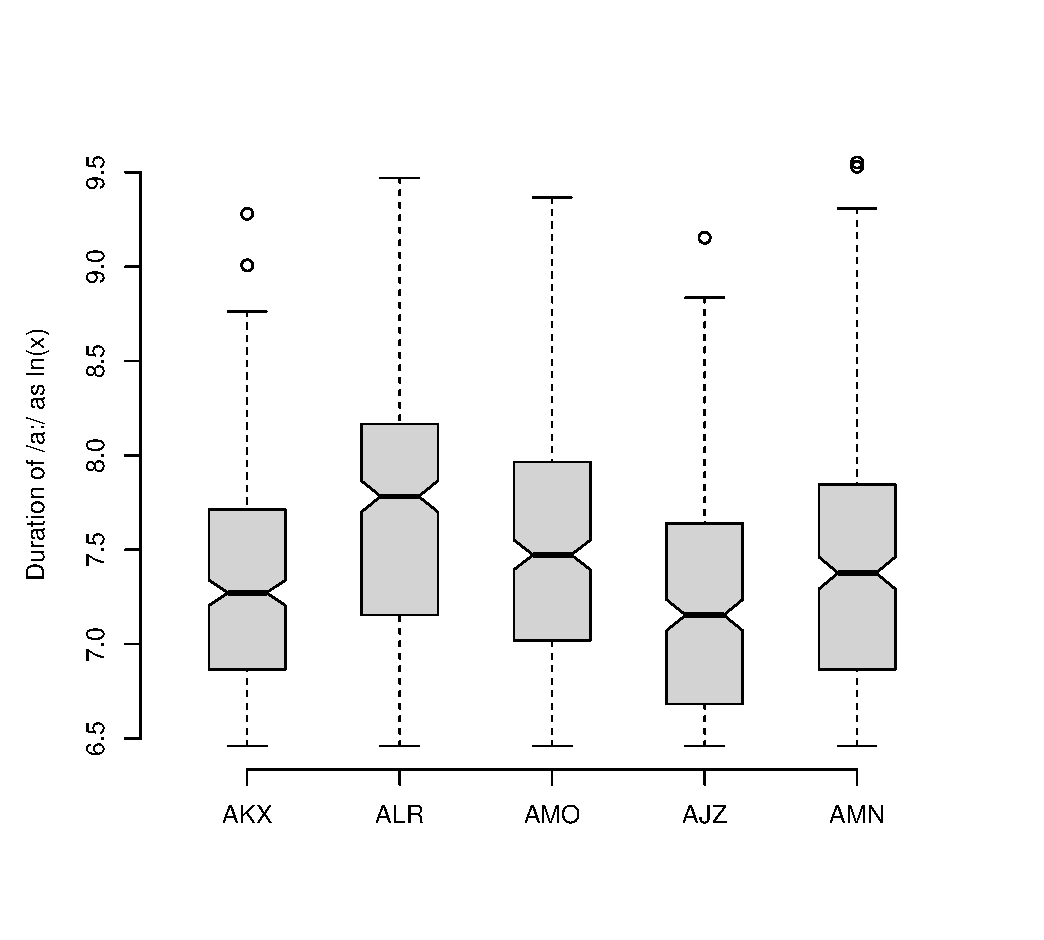
\includegraphics[width=0.6\textwidth]{../Graphen/Duration_of_a_5speakers.eps}
	\centering
	\caption[Phoneme length variation between speakers]{Overview of \texttt{/a:/} length on the 5 most frequent speakers. Phoneme length is expressed as the natural logarithm of the sample frequency. While the minimum duration is technically limited to an equal value corresponding to 0.04 sec, all other coordinates vary, e.g. maximum value has a variation of 0.14 sec between speakers AKX and ALR. The greatest median variation is 0.07 sec between speakers ALR (0.15 sec) and AJZ (0.08 sec).}
	\label{fig:speaker_cmp}
\end{figure}

\chapter{Phoneme durations and the dynamics of speech}
The phoneme inventory used in Verbmobil includes 52 classes defined according to the German SAMPA. Using the classical phonetic conventions, we can group these phonemes on a first level according to their phonetic features using a tree structure into vowels, consonants and a glottal stop, although the latter one is sometimes treated as a consonant \cite{Kohler1995}. Vowels represent 24\% of the total phoneme inventory analyzed. Further relevant groupings are being examined under sections ``Vowels`` and ``Consonants``.

Pauses may be caused and/or be quantitatively modified both by linguistic (e.g. phonological) and non-linguistic factors, like technical, psychological, dialog dynamics, etc. Consequently pause length variation needs to be treated separately from phoneme duration variation, as a not negligeable large set of other factors are to be considered for this, which extends beyond the purpose of this work.

The literature records on many potential influencing factors for the duration of phonemes, which vary not only from one author to another but also from one language to another. For the German language, intuition aside, we have information on such factors provided by: Kohler \cite{Kohler1992}, Riedi \cite{Riedi1995}, Moebius \cite{Moebius1996}, and Brinckmann \& Trouvain \cite{Brinckmann_2003}, who applied some of the existent segment duration models to the German language.

As we recreated the tree model of Brinckmann \& Trouvain \cite{Brinckmann_2003} for the most part, we also selected most of the features used by them. Here just a rough listing of these factors:

\begin{itemize}
	\item phoneme id
	\item vowel and syllable stress
	\item manner of articulation for consonants
	\item position of phoneme in syllable
	\item position of syllable in word
	\item position of word in turn
	\item part-of-speech: function word, content word, proper name, interjection-or-answer-particle
	\item speech rate
\end{itemize}

A detailed description of the model implementation and phoneme features used follows in Chapter 6.

\section{Vowels}
Vowels are an important class, because their variation in terms of duration correlates well with the speech rate. One can say that vowels generally tend to get proportionally longer when the words themselves are spoken slower. We obtained an overall correlation coefficient of 0.72 for vowels against speech rate. Inside the vowel group we could identify the primary stressed vowels as the actual correlation owners, with a group correlation value of 0.75, while the unstressed and secondary stressed ones showed rather modest correlation values of 0.56, resp. 0.47. 

We identified following vowel categories as being relevant for our purpose:

\begin{itemize}
	\item Diphthongs represent two vowels that are articulated together in a syllable. They are generally characterized by longer durations. German knows three diphthongs: \texttt{/aI/, /aU/} and \texttt{/OY/} as in \textit{Haus} \texttt{/haUs/},  \textit{heiß} \texttt{/haIs/} and \textit{moin} \texttt{/mOYn/}. We considered them as a separate group, as they are generally longer than all other phonemes.
	\item Schwa: most frequent vowel in German as well as in English. It is also called a reduction vowel \cite{Kohler1995}, as most of the other monophthongs tend to be articulated as schwa in non-stressed vowels. Verbmobil differentiates two types of schwa for the German language: \texttt{/@/} like in the last syllable of \textit{lesen} and \texttt{/6/} like in \textit{Leser}, where the reduced vowel is followed by an \texttt{/r/}.
	\item Long vowels. As long vowels usually carry the primary stress, as some german phonetics manuals such as the one of Kohler \cite{Kohler1995} suggest, we considered the long vowels as a standalone subclass of vowels. The correlation value for the long vowel group is even greather than that of the primary stressed one, amounting to 0.79.
	\item Short vowels in opposition to the above mentioned vowel categories.
\end{itemize}

\section{Glottal stop}
The glottal stop occurs 13 348 times and only word initially in our database, marked with \texttt{/Q/}. We decided to treat it separately because of its particular usage in German: it may occur only at the beginning of a word or a word stem and in front of a vowel. Some phonetic manuals don't event consider it a phoneme \cite{Ternes2012}. Furthermore, it's acoustical properties make it look like a (filled) pause in speech, as you may see in Fig. ..., which represents a challenge for the transcription. As our files were segmented automatically, there is place for doubt about the accuracy of the collected data for \texttt{/Q/}.

However, unlike pauses we did consider it  for analysis, as it is has an important communicative function as delimiter for words and morphemes. It is in fact one of the important clues which help hearer understand speech \cite{Ternes2012}. 

The information collected from our database show a very large variation of it's duration from 0.04 sec. to 2.05 sec., with $\sigma = 0.06$, consistent with the official data on the complete VMII. However, if we remove the upper 0.8 \% of the duration data, we obtain a dataset having only half of the mentioned variation with $\sigma = 0.03$ and a maximum duration of 0.3 seconds. We checked manually some of the largest outliers and they proved to be a result of wrong segmentation. Their real duration was within the first 2 thirds of the data.

\section{Consonants}
Based on the correlation between phoneme duration and speech rate we created a subgroup of consonants containing the nasals and \texttt{/x/, /C/, /h/} with a relatively good correlation value $\geq 0.7$, and considered plosives to be a subgroup because of their consistently low correlation $\leq 0.42$.

A big surprize in the Verbmobil dataset was the huge duration variation of the plosive /t/, which was even greater than most of the fricatives. Evaluation of some samples showed this to be a result of wrong segmentation in the context /ts/, giving /t/ the longer duration and /s/ the shorter one. Another explanation would be that the phase before the release phase may indeed be relatively long.

Below an overview of the classical consonant categories.
\begin{itemize}
	\item Plosives, which are generally short, is due to their articulation characteristics.
	\item Fricatives, which show a legth variation almost comparable to that of vowels.
	\item Nasals: /m/, /n/, /N/.
	\item Specials: /h/, /l/, /C/, /j/, /r/
\end{itemize}


\chapter{Defining speech rate}
Under speech rate or speech tempo we understand a measure of how fast someone speaks. This may be seen as a discrete variable, with discrete values as \textit{slow}, \textit{normal}, and \textit{fast} or as a continuous one, with continuous numerical values.  We opted for the continuous version, as it is better suited for our purpose.

Expressed mathematically, this would be a fraction of something divided by total time ocupied by that something. The German word ``Sprechgeschwindigkeit`` involves the concept of ``speed`` in the equation, which would be space divided by time. In the case of speech this would be number of units divided by total time ocupied by those units. This is fine, if one has a fixed time interval and is interested in the number of units that may fit in. However, this way of looking at it does not consider the fact, that the length of the unit may vary. We are not interested in variing the number of units, which should actually stay constant. We are rather interested in variing the time interval while keeping the number of units constant. This is what happends when someone is speaking faster or slower than a specific norm. Therefore we inverted the typical speed-like calculating formula, as you can see in Eq. \ref{eq1}, so we can investigate the length variation in the speech units, with focus on units = phonemes.

\begin{equation}
\label{eq1}
	SR = \frac{segment \quad duration}{unit\quad count}
\end{equation}

The next thing to think about is the size and identity of the fraction elements. Unit size may be phoneme, syllable or word. Variing the scope from local to globa, the segment on which we calculate speech rate may be a syllable, a word, a phrase, a speech turn or the entire corpus. In the literature \cite{Pfitzinger1998} we also found mentions about a relative speech rate, which combines the speech rate calculated to two different unit sizes.

From the beginning, we did not consider the variant of calculating a speech rate for the entire corpus. Given its structure of dialogues recorded by many speakers, it is straightfoward that speech rate may vary tremendousely not only between speakers, but also between different speech turns, and consequently be a bad measure for characterizing our corpus. The size of a speech turn in a dialog proved to be a bad measure as well. The reason for this is again the nature of spontaneous speech as ``live`` creation of the human mind. Hesitations, thinking, and emotions have a much greater influence as in read speech, and result in a variing tempo at which we produce speech. In figure \ref{fig:SR_example} we are illustrating an example of this phenomenon.

\begin{figure}[htbp]
	\centering
	\noindent\makebox[\textwidth]{\includegraphics[width=\paperwidth, clip]{../Graphen/SR_example.eps}}
	\vspace{-25mm}
	\caption[Example of speech rate variation inside a turn]{This is the content of the speech turn number 22 of speaker AAJ in dialoge g001. The closer the points are to oneanother, the faster he speaks. Orange lines mark prosodic boundaries.}
	\label{fig:SR_example}
\end{figure}

Seing this, there is no wonder that we got no good correlation values as long as we calculated speech rate on entire turns. This got better when we reduced the size of the segment to phrase, and then further down to words. 
An additional measure we used to evaluate how well a speech rate calculating formula may suit our purpose was the correlation value between speech rate and phoneme duration. As long vowels proved to be the most sensible to the variation of the speaking tempo, we present below the values we obtained for this group, together with the speech rate calculated at different segment sizes.

\begin{table}[htbp]
\caption {Duration of long vowels vs. speech rate calculated at turn, phrase, and word level} 
%\centering
\vspace{10mm}
\begin{tabular}{|l|l|c|}
\hline
Segment	 & Formula & Correlation coefficient (Pearson)\\
\hline
\hline
Turn 		& $turn\_dur / phon\_count$ &0.727178570436 \\
	\hline
	&  $phon\_count / turn\_dur$ & -0.270392865503 \\
	\hline
Phrase  & $phrase\_dur / phon\_count$ & 0.561266362391\\
	\hline
	&  $phon\_count / phrase\_dur$ & -0.377058296098\\
	\hline
Word  & $word\_dur / phon\_count$ &  0.794901825792\\
	\hline
	&  $phon\_count / phrase\_dur$ & -0.616539202577\\
	\hline
\end{tabular}
\end{table}

\begin{figure}[htbp]
\centering
	\begin{subfigure}[h]{0.48\textwidth}
	\centering
	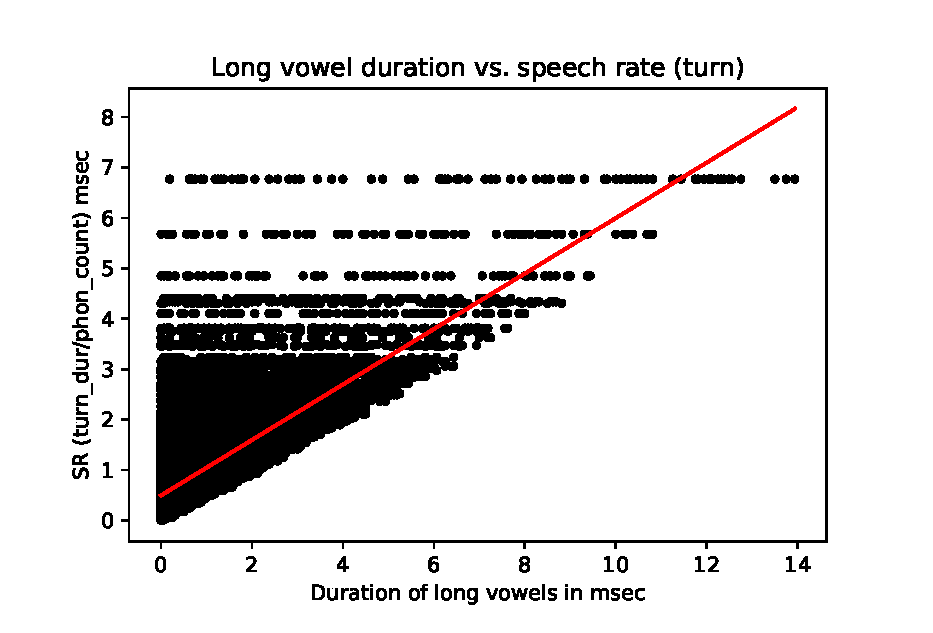
\includegraphics[width=\textwidth]{../Graphen/SR_turn.eps}
	\label{fig:tsr}
	\end{subfigure}
\hfill
	\begin{subfigure}[h]{0.48\textwidth}
	\centering
	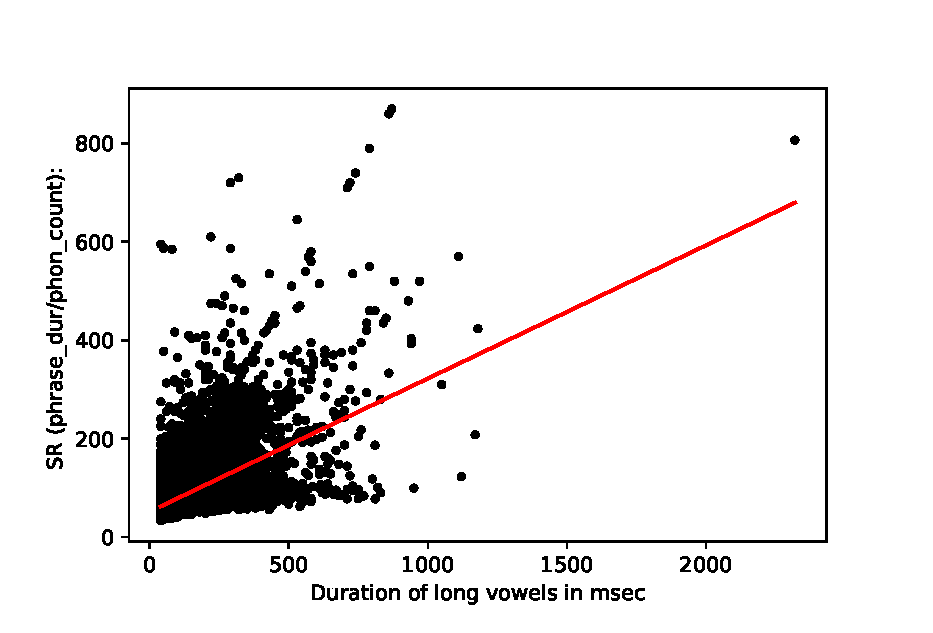
\includegraphics[width=\textwidth]{../Graphen/SR0.eps}
	\label{fig:phraseSR}
	\end{subfigure}
\hfill
	\begin{subfigure}[h]{0.48\textwidth}
	\centering
	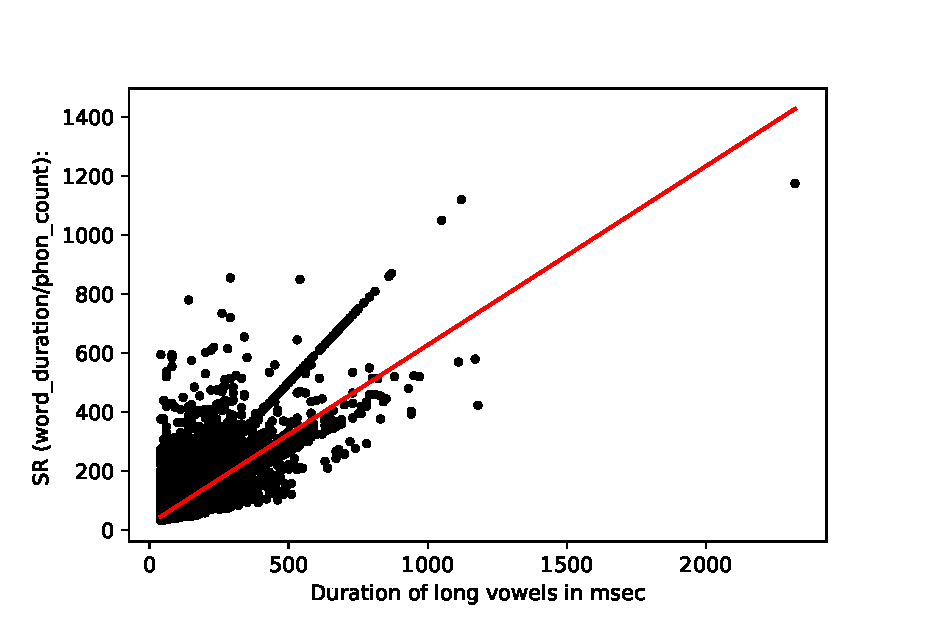
\includegraphics[width=\textwidth]{../Graphen/SR4.eps}
	\label{fig:wsr}
	\end{subfigure}
\caption[Speech rate vs long vowel duration]{Phoneme durations measured in msec plotted against different speech rates.}
\label{fig:SR_corr}
\end{figure}

\chapter{Phoneme duration prediction models}
There are several duration prediction methods in use: 
\begin{itemize}
	\item Klatt \cite{Klatt1979} is a rather simple method developped originally for American English. It multiplies a so-called inherent duration of given segment with a context dependent factor value and adds this to a segment specific minimal duration. Then the duration is estimated by adjusting the change coeficient successively for different factors, 11 of them being suggested by Klatt. These account for 84\% of observed total variance in segmental durations. The challenges of using this method reside in finding an appropriate inherent duration, adapting the Klatt factor values to the German language, and chosing the minimal duration to use.
	\item CART \cite{Riley1992} is a binary classification and regression tree with questions about the influencing factors at nodes and predicted values at the leaves. It allows consideration of both categorical and continuous factors, is quite simple and easy to interpret, in contrast to e.g. neural networks, and has a good time complexity of N*logN. The challenge of selecting an appropriate feature set is solved statistically. One drawback is that it needs a huge amount of training data in order to perform well. Also its performance deteriorates significantly with noisy or sparse training data \cite{Moebius1996}.
	\item Sums-of-products (SoP) proposed by van Santen \cite{Santen1994} generalizes the formula proposed by Klatt and uses a decision tree to group factors acting in the same direction, either lengthening or shortening the phonemes, so their effects add up (amplificatory interactions). In fact, the most important part and main challange of this model is to find an appropriate combination of factors to be used for specific phoneme groups. He didn't use speech rate as a factor, but observed that the performance of the model deteriorates when the speech rate changes. The advantage of this solution is that is copes well with noisy or missing data, and works well with much less training data than CART \cite{Moebius1996}. The application of this model for the German language by Möbius and van Santen using the PhontDat database resulted in an overall correlation coefficient of 0.896.
	\item Neural networks. Riedi \cite{Riedi1995} implemented a feed-forward neural network with two hidden layers for the prediction of phoneme durations and obtained a slightly better correlation coefficient than CART of 0.89 vs. 0.86.
\end{itemize}

Brinckmann and Trouvain \cite{Brinckmann_2003} compared Klatt and CART methods for predicting segment duration using the PhonDat database. Their results show a significantly better performance of CART over Klatt, with values of 0.86 vs. 0.79 for the correlation coefficient, consistent with previous results. However, they also report a strong influence of  the quality of the input data on the model performance.

\section{Method}
Whichever phoneme duration prediction model one takes, and whichever size of the segment one takes in the denominator, in terms of syllable, word, foot or phrase duration... Larger the segment size, larger the number of influencing factors for phoneme duration. We opted for a progressive approach, starting at the syllable level ?.

Our approach is based on the observation that specific phonemes, respectively phoneme groups, occupy a specific percent of the total word duration (fig. \ref{fig:boxplot_genau}), and that certain phonemes seem to modify their duration according to that of the segment they're in to a much higher degree than others, as you can see in fig. \ref{fig:w_dur_vs_pho}.

\begin{figure}[htbp]
	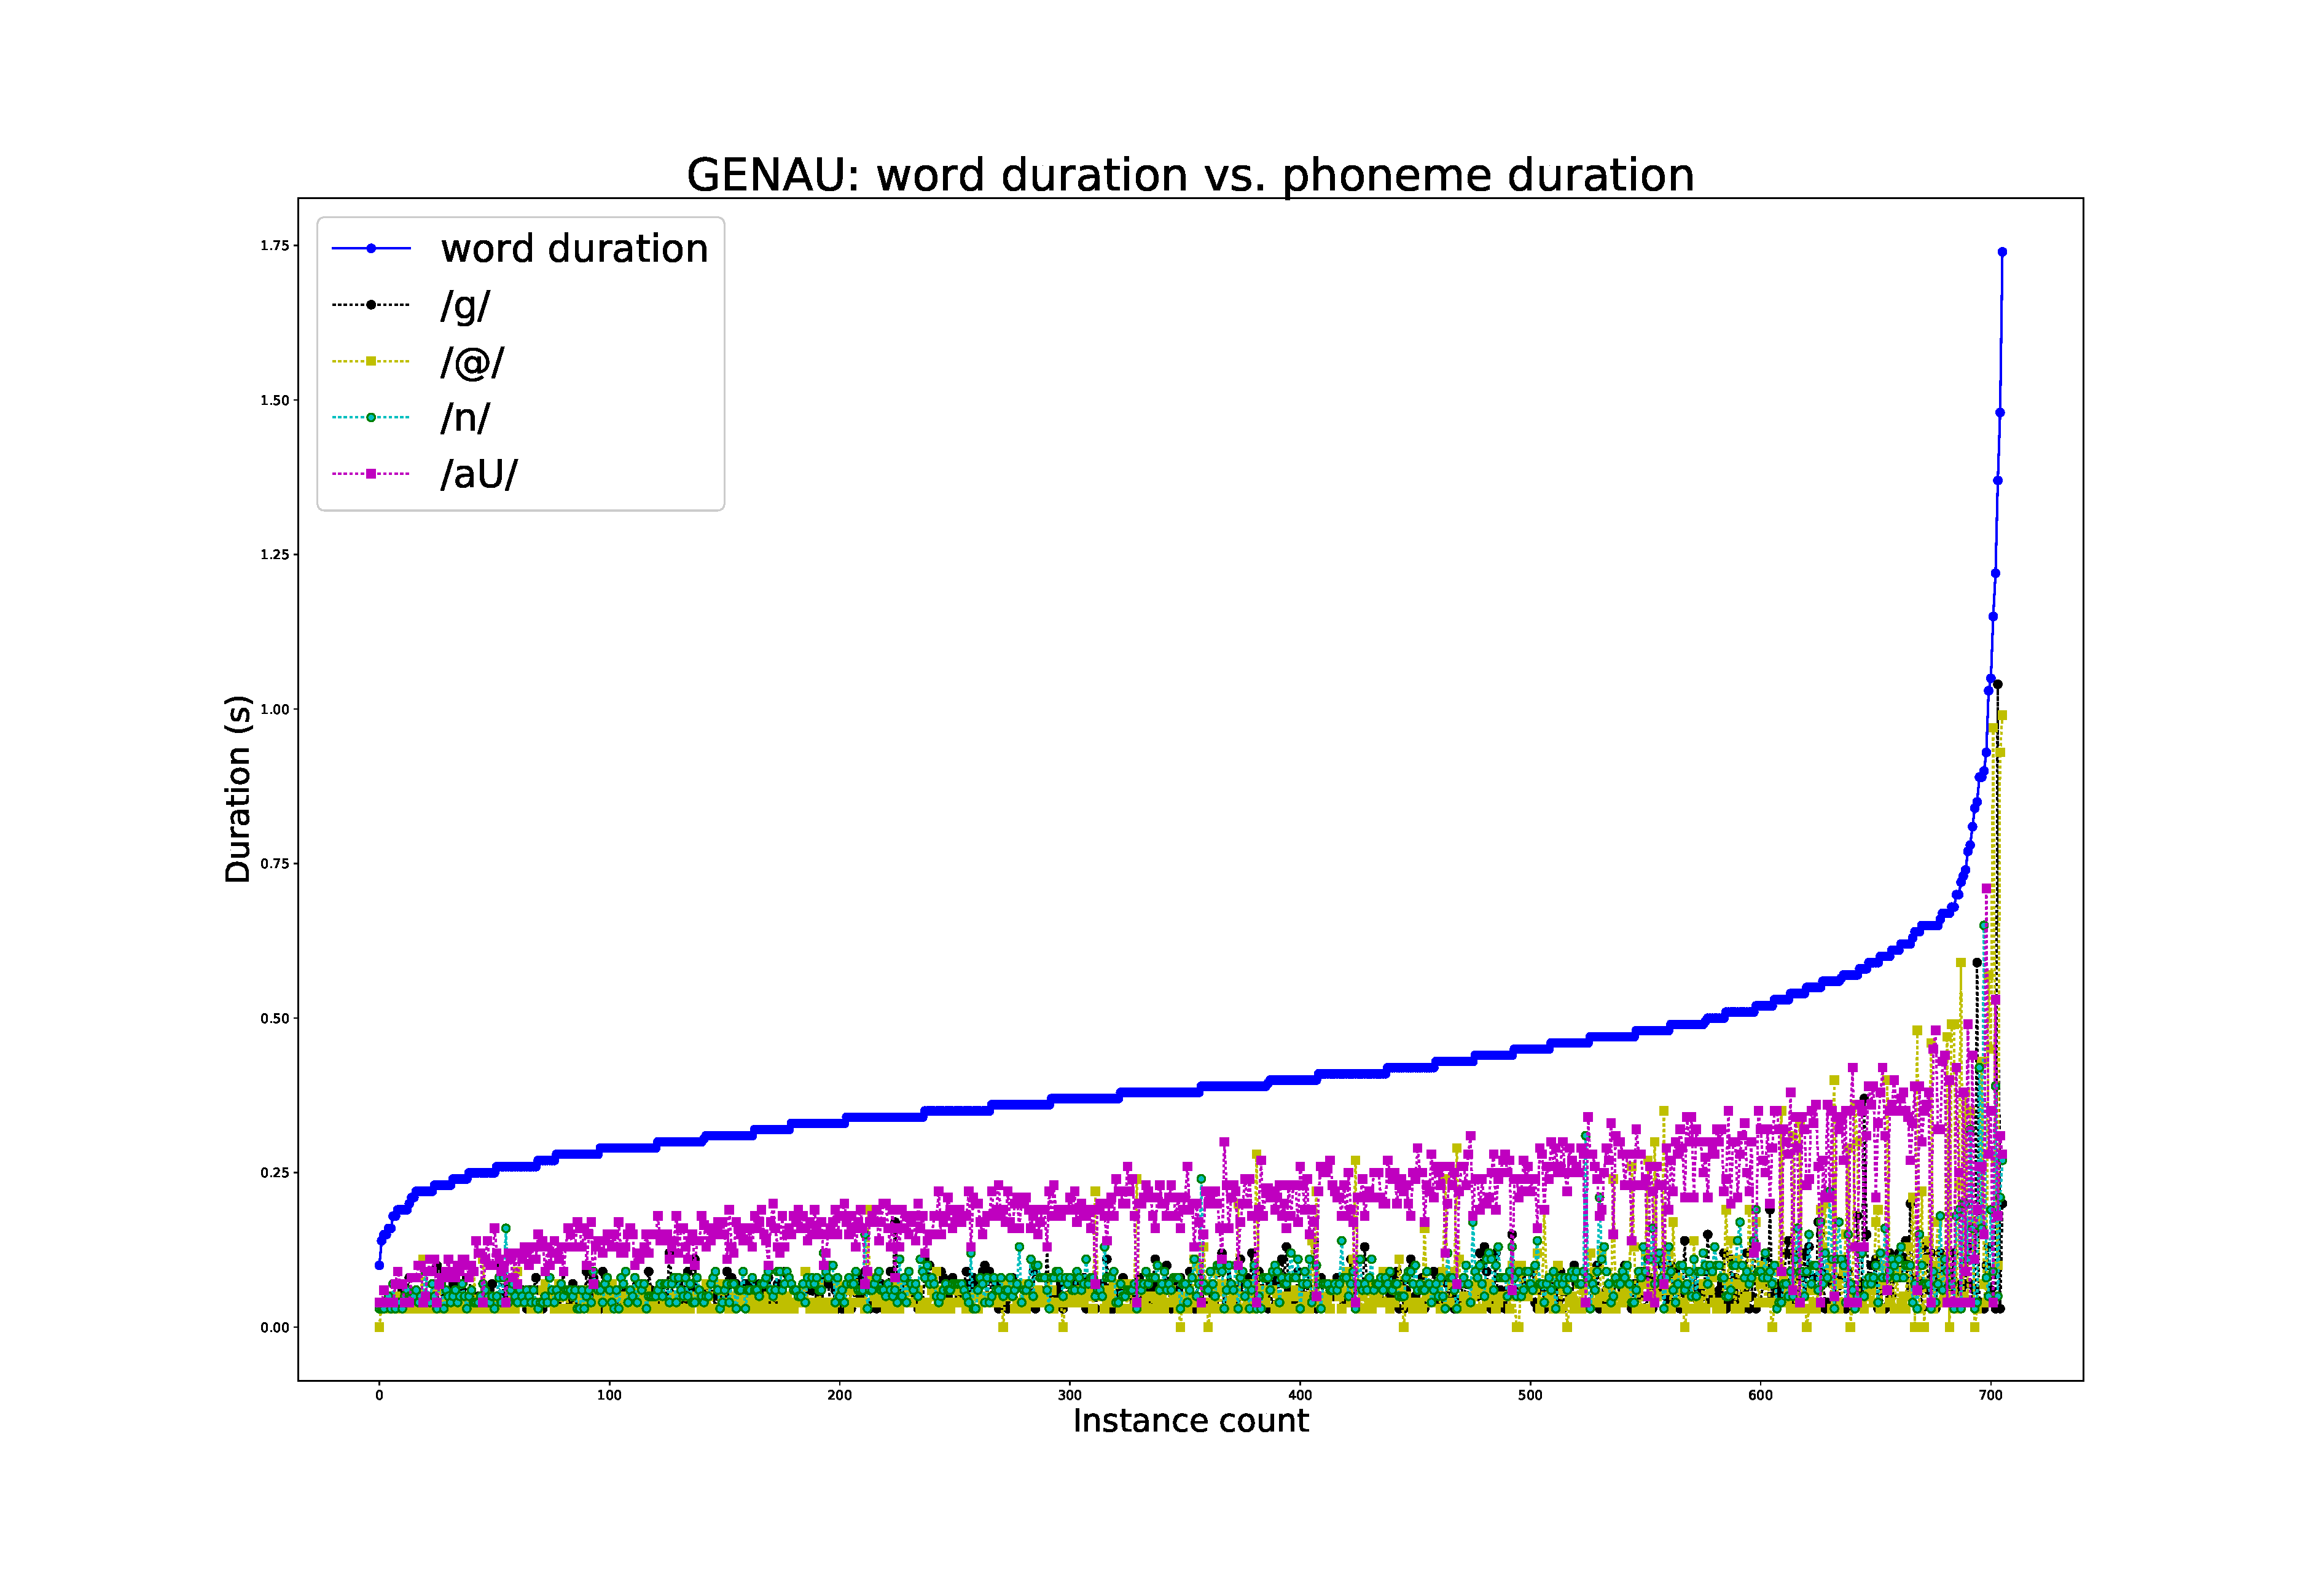
\includegraphics[width=\textwidth]{../Graphen/Stats_for_genau.eps}
	\centering
	\caption[Word duration of ``genau`` vs. its phoneme durations]{We ordered ascendingly the 706 occurences of the word ``genau`` based on word duration and ploted recorded durations of the component phonemes against it. The picture suggests clearly that the diphthong \texttt{/aU/} occupies a rather fixed steak of the total word duration, while the others show no adjustment to the increasing word total duration. }
	\label{fig:w_dur_vs_pho}
\end{figure}

\begin{figure}[htbp]
	\includegraphics[width=.55\linewidth]{../Graphen/Sound_boxplot_genau.eps}
	\centering
	\caption[Phoneme proportions in ``genau``]{Proportions taken by the component phonemes of ``genau`` suggest the possibility of grouping them in disjunct classes. Here we explored the phoneme distribution for a relatively short occurence of our reference word, of only 0.3 sec found 25 times. This one, as well as others, correlates well with the overall phoneme distribution on all occurences.}
	\label{fig:boxplot_genau}
\end{figure}

\chapter{Conclusion and Outlook}
Our model calculates an approximation for the phoneme duration when its corresponding speech segment changes in terms of duration. It does this no matter what was the cause of the duration change in the segment. However, when speech rate changes, there are also other speech characteristics, like prosody and phoneme quality which change, and which cannot be simulated only by modifying the phoneme duration. Therefore, making speech sound natural while modifying the speech rate needs to consider and adjust these other features too.

Koreman showed \cite{Koreman_2006} that the perceived speech rate is also influenced by the listener's knowledge of the expected articulations for a particular utterance, therefore it makes a difference if all expected phones are also articulated or not. Consequently, one could compare speech rate considering only articulated vowels/syllables, as well as considering both realized and intended syllables, and test both methods with a given model. One possible result of such an approach would be the prediction of phonemes reaching $duration = 0$ at specific speech rates, which means predict phoneme drop phenomena.

\subsubsection*{Notizen}
Analyze duration changes of vowels in interrupted words.
Consider actual realized syllables in speech instead of syllables based on the canonical transcription?. In spontaneous speech, the word and syllable boundaries change, and this change influences other phonetic aspects such as stress, syllable duration, phoneme duration.

\printbibliography
\end{document}